\documentclass[11pt,a4paper,oneside]{article}
\renewcommand{\baselinestretch}{1.2}
\usepackage{sectsty,setspace,natbib,wasysym} 
\usepackage[top=1.00in, bottom=1.0in, left=1in, right=1.25in]{geometry} 
\usepackage{graphicx}
\usepackage{latexsym,amssymb,epsf} 
\usepackage{epstopdf}
\usepackage{amsmath}
\usepackage{hyperref}

\graphicspath{{/Users/megan/Documents/GitHub/temporalvar/figures}}

\newenvironment{smitemize}{
\begin{itemize}
  \setlength{\itemsep}{1pt}
  \setlength{\parskip}{0pt}
  \setlength{\parsep}{0pt}}
{\end{itemize}
}

\usepackage{fancyhdr}
\pagestyle{fancy}
\fancyhead[LO]{December 2013}
\fancyhead[RO]{Variable environments \& climate change}

\begin{document}
\renewcommand{\labelitemi}{$-$}
\title{Coexistence and climate change: \\The role of
    temporal-variability in structuring future communities \\Updating To Do List from Skype Meetings}
    \author{Wolkovich \& Donahue}
\date{Last updated: 26 Aug 2014}
\maketitle

\newpage
\tableofcontents

\section{Notes}
\subsection{Skype Meeting - August 24, 2014}
\begin{itemize}
\item Running PhenologyModel.R does not produce coexistence even with two species set with the same parameters as Chesson et al 2004.  In Chesson et al 2004, species' biomasses bounce around 0.2.  Our sims drop to very low numbers by year 30.  Why?
\item Previous sims which stepped thru within year dynamics resulted in coexistence
\item Tried: decreasing extinction threshold to 1/100000 from 1/10000.  This does increase persistence (obviously) but does not change the pattern of species bouncing at very low densities
\item Tried: increasing the within-season time to 8 days from 5 days.  I did this because the in some years it wasn't clear from the plots (I did not check the numerics) that the species had reached max biomass.  Not clear that this had any effect.
\item Compared to Chesson: there are a few details of the simulation that aren't clearly laid out in Chesson et al 2004.  Particularly, it isn't clear when "flowering" occurs.  That is,  when is the end of the season?  we take the max biomass of each species, but could have a set flowering time for both species (say, when R<R*).  However, I think we have made a reasonable choice here and that, while it might result in differences with Chesson et al 2004, it should not result in the problem at hand.
\item Things to look at: what does R-uptake look like within a season?  Does it match the patters in Fig 2 of Chesson et al 2004?
\item: To do: when preparing for ASN, I changed the within-year simulation from a for-loop to an ode solver.  I did this because the within-season step size needed to be adjusted for differences in initial biomass and resource level: if step size was small enough to catch the crossing of the Rstar threshold, then it took forever the rest of the season.  However, I never completed the comparison of the ode solver and the within year for-loop.  That is the next task
\end{itemize}

\subsection{Megan: September 8, 2014}

\begin{figure}[h!]
\centering
\noindent 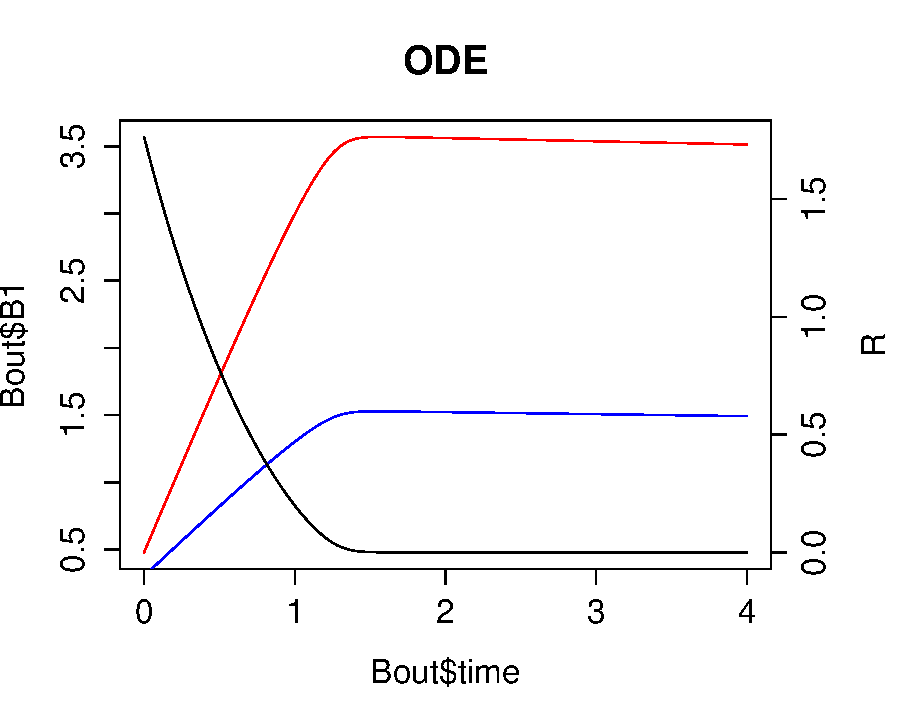
\includegraphics[width=0.8\textwidth]{/20140908_1122am_ODEplot.png}
\caption{{\bf Compare ODE and StepStep solutions to our equations}}
\end{figure}

\begin{figure}[h!]
\centering
\noindent 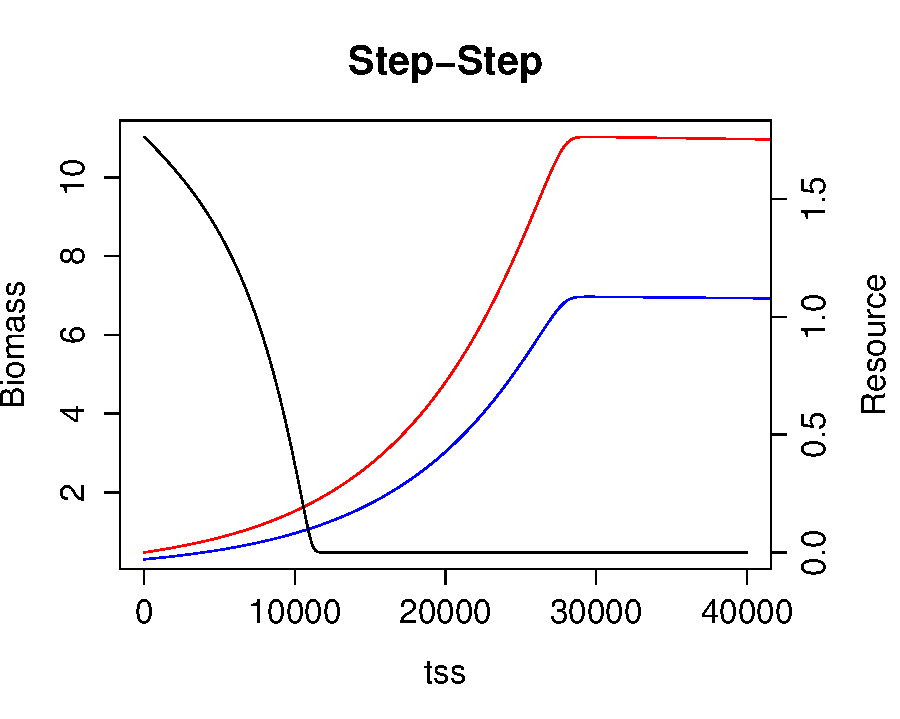
\includegraphics[width=0.8\textwidth]{/20140908_1122am_StepStepPlot.png}
\caption{{\bf Compare ODE and StepStep solutions to our equations}}
\end{figure}


\end{document}

